\section{Bluetooth}

\begin{figure}[H]
\begin{center}
	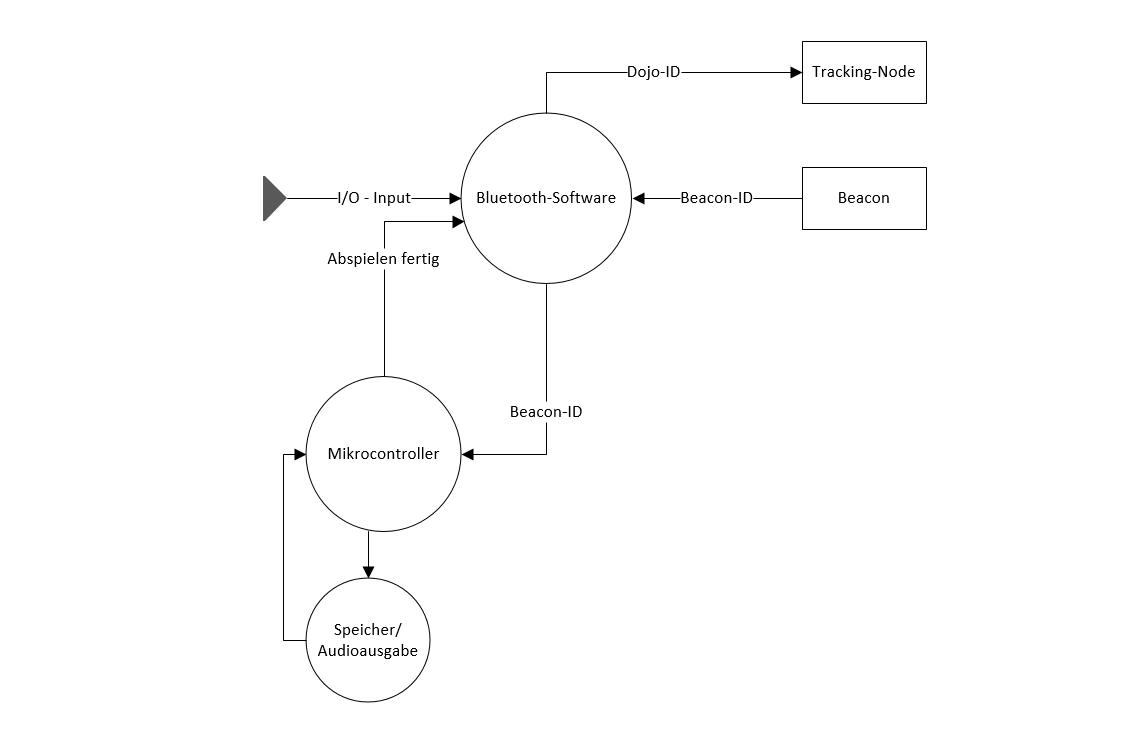
\includegraphics[width=160mm]{data/Bluetooth.png}
	\caption{Grobstruktur der Bluetooth-Software} %picture caption
	\label{fig:first_layer}
\end{center}
\end{figure}

Obenstehendes zeigt die Grobstruktur der Bluetooth-Software. Der Benutzer drückt eine für diese Funktion definierte Starttaste (Input), welche das Suchen von Bluetooth Signalen in der Nähe auslöst. Vom Beacon mit dem stärksten Signal wird dann die Beacon-ID empfangen. Diese Beacon-ID wird Software-intern weitergeleitet, um das dazugehörige Audio-File abzuspielen. Während des Abspielens der Audio-File ist die Funktion der Starttaste deaktiviert, um Überschneidungen von Programmabläufen und daraus resultierende mögliche Fehler zu minimieren. Nach dem Abspielen einer Audio-File wird die Funktion der Starttaste wieder aktiviert. Für ein mögliches Einbinden des Dojo in ein Tracking-System wird der Dojo in der Lage sein, seine eigene Erkennungsnummer auf Anfrage zu senden, ähnlich wie ein Beacon.
\subsection{Schnittstellen zu anderen Bereichen:}
Dojo soll, um Energie zu sparen, erst per Knopfdruck das Kunstobjekt mit der stärksten Signalstärke suchen und die entsprechende Datei dafür abspielen. Dies führt Software-intern zu einer Parameterübergabe an die Audio-/Speichersektion.
Während der Audiowiedergabe soll das BT ausgeschaltet bleiben, weshalb wiederum Software-intern eine Parameterübergabe bzw. -Abfrage erfolgen muss. Dies soll verhindern, dass während der Audio-Wiedergabe das Suchen und Abspielen eines weiteren Objekts möglich ist.
Beim Wunschziel Daten-Austausch herrscht eine enge Verbundenheit zwischen BT und Speicher.
